\chapter{Training process of Convolutional Neural Networks}\label{ch:cnn_train}
Three Convolutional Neural Networks (CNNs) were trained throughout this analysis. There are differences to each CNN and will be described fully in the next sections but the main difference are the amount of particle images used for training and validation. CNN1075 used 1,075 muons and 1,075 pions for training and the same amount of each particle for validation. CNN10000 used 10,000 muons and 10,000 pions split in half for testing and training. Lastly CNN100000 had muons, pions, protons, electrons, and gammas in it's training and validation set. Each particle had 20,000 images and training and validation was split $90\%$ training, $10\%$ validation. This chapter will also describe the different hardware frameworks used for training beginning on a CPU and ending on a GPU cluster. 


%\section{Hardware Frameworks used for Training}
%\subsection{Syracuse CPU Machine setup}
%\subsection{Syracuse University GPU Cluster Setup}


\section{Hardware Configurations for Convolutional Neural Network Training}\label{research approach}
The first training iteration, CNN1075, was a proof of concept. This CNN was trained on my local machine for \sim 4-5 weeks. The batch size had to be very small as well as the image size due to the lack of computation resources. The second iteration of training, CNN10000, was trained on a Fermilab stationed Syracuse University machine. This machine had 6 TB of disk space, 6 cores at 2.1 GHz and 32 GB of RAM. The use of this machine allowed me to increase the training sample as well as the batch size and hence further increase the accuracy of the neural network. Lastly, the CNN100000 was trained using two GTX 1080 Ti GPUs with 11GB of memory on a node on the Syracuse University GPU cluster, SUrge, that has 8 cores and 16GB of memory. This increase in memory as well as the capability to use 2 GPUs drastically cut down on training time from \sim 4-5 weeks to \sim 8 hours. SUrge also allowed for hyperparameter optimization by being able to run multiple training iterations over the two GPUs. Lastly, SUrge allowed for training over higher resolution images and a larger particle class of 5 particles vs 2 particles. 

\section{Creating images using LArTPC data for training/validation of CNNS}\label{image_making}
The $\mu/\pi$ image dataset used to train and validate CNN1075 was created using single generated isotropic muons and pions from 0-2 GeV energy range. 2,150 muons and 2,150 pions were used for training and testing split 50\%. The images were created using LArSoft, a liquid argon software, and were based on wire number and time tick in the collection plane. Uboonecode reconstruction version v05{\_}08{\_}00 was used. The raw ADC value after noise filtering was the wire signal. Each collection plane greyscale image was 3456x1600x1 where 6 time ticks were pooled into 1 bin. 

After the image was created, the region of interest (ROI) in the image was found by using Open CV, a image processing open source software package, to scan the image starting from the edges and stopping once a bright pixel is encountered. At this step, the ROI can be larger or smaller than the necessary size of a training image and the XY ratio of the image is not kept. This ROI is then resized to an image of 224x224x1. 

The greyscale color standard is 8bit therefore the ADC value of wire and time tick was also downsampled due to the 12bit ADC value MicroBooNE has. To do this, the highest ADC pixel in the image was found and then this was divided by the rest placing all pixel values between 0-1. From there, all pixel values are then multiplied by 255.

The $\mu/\pi$ image dataset used to train and validate the CNN10000 was also created using single generated isotropic muons and pions from 0-2 GeV energy range. 10,000 muons and 10,000 pions were used for training and testing split 50\%. Uboonecode v06{\_}23{\_}00 was used instead of v05{\_}08{\_}00. Each collection plane greyscale image was 3456x1280x1 where 5 time ticks were pooled into 1 bin which is different than the previous dataset and was implemented due to the fact that the time ticks of an event went from 9400 to 6400 with the change of uboonecode version. Issues that arose in CNN1075 that were fixed in CNN10000 include zero-padding images in X and Y that are smaller than 224X224 to eliminate over-zooming effect and fixing a bug that shifted pixels separated by a dead-wire region.

The $\mu/\pi/p/e/\gamma$ image dataset used to train and validate the CNN100000 were created using single generated isotropic particles with energy range from 0-2 GeV. 20,000 of each particle were used for training and were split 90/10 between training and testing sets. Uboonecode v06{\_}23{\_}00 was used for these images. The collection plane greyscale iamge had the same dimensions as CNN10000, 3456x1280x1 and the ROI algorithm was the same except for resizing these images to 576x576. 

A major change other than the higher resolution images was the treatment of the ADC values. In the first two image making schemes, the highest pixel value was found per image and the image was then normalized by that. The issue arising from this ADC normalization wasn't inherent in $\mu/\pi$ training due to the fact that both particles are minimum ionizing particles in liquid argon, however, when dealing with a larger particle class, it was necessary to try and make sure energy deposition by each particle was preserved. The energy deposition in a particle image corresponds to the ADC value or pixel brightness. To preserve energy deposition, the ADC float value was passed straight to the image rather than doing any image normalization. This then makes sure that minimum ionizing particles like muons and pions appear dimmer than highly ionizing particles like protons.  

Images were also made from BNB+Cosmic events that passed the cc-inclusive selection 1 filter right before the 75 cm track length cut and were classified using the CNN10000. The dataset used to create these images is the same one used in \cite{cc-inclusive}, \textit{prodgenie{\_}bnb{\_}nu{\_}cosmic{\_}uboone{\_}mcc7{\_}reco2}. These images were created using information from the track candidate that passed the filter. Only wire number and time ticks associated to the track candidate were drawn on the image to mimic a single particle generated image. 

These images were then classified using CNN10000. Two approaches were taken in making these images. The first was using the image normalization above where the maximum pixel in each image is used as a normalization constant to get all pixels between 0-1 then multiply all pixels by 255. As described above, this is the incorrect way to normalize. The second way the images were created was by passing the ADC float to the image. The results of CNN10000 performance are shown in section \ref{research approach}. 

Lastly, multiple BNB+Cosmic images per event were made for CNN100000 by reducing many of selection I cuts to try and let the CNN do particle as well as event identification. This image making scheme used for CNN100000 will be described in more detail in later sections. 

\section{Convolutional Neural Network Training}
\subsection{Training CNN1075}
The results of CNN1075 are described in this section. The accuracy is how well CNN1075 is doing by epoch and was 74.5\%. The loss is gradient descent or minimization of the error of the weights and biases used in each neuron of each layer of CNN1075 and was 58\% with a trend sloping downwards on the loss curve as well as a trend sloping upward in the accuracy curve. The accuracy and loss of CNN1075 are shown in figure \ref{fig:loss_accuracy_1075}. Due to the depth of the neural network framework, it was necessary to train with a larger dataset and for more epochs, however, the downward slope of the loss curve is an indication that once trained for longer with a higher training sample, neural networks can be used for $\mu/\pi$ separation. The hyperparameters used to train CNN1075 are detailed below: 

\begin{multicols}{3}
\begin{itemize}
 \item \textit{train{\_}batch{\_}size: 50}
 \item \textit{test{\_}batch{\_}size: 50}
 \item \textit{test{\_}iter: 50}
 \item \textit{test{\_}interval: 50}
 \item \textit{base{\_}lr: 0.01}
 \item \textit{lr{\_}policy: "step"}
 \item \textit{gamma: 0.1}
 \item \textit{stepsize: 200}
 \item \textit{display: 50}
 \item \textit{max{\_}iter: 5000}
 \item \textit{momentum: 0.9}
 \item \textit{weight{\_}decay: 0.0005}
 \item \textit{snapshot: 100}
\end{itemize}
\end{multicols}

\begin{figure}[htp!]
\centering
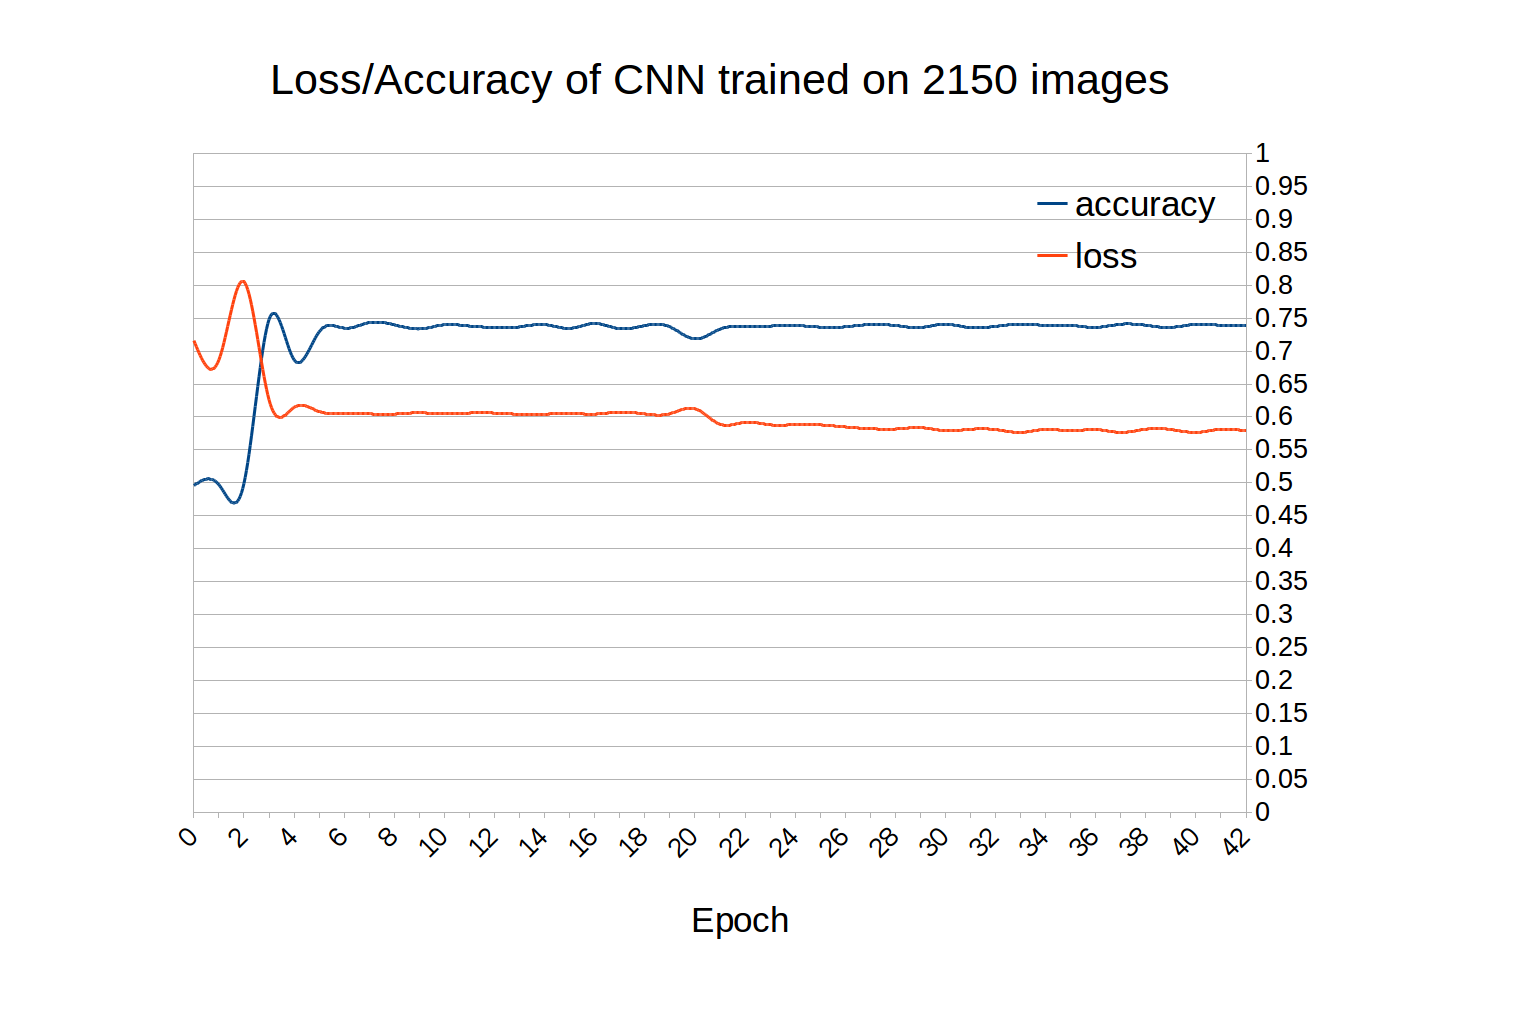
\includegraphics[width=\textwidth]{figs/acc_loss_CNN1075.png}
\caption{Accuracy vs. Loss of AlexNet 2-output $\mu/\pi$ sample consisting of 2,150 images each.} 
\label{fig:loss_accuracy_1075}
\end{figure}


\begin{figure}[htp!]
\centering
	\begin{subfigure}[b]{.68\textwidth}
	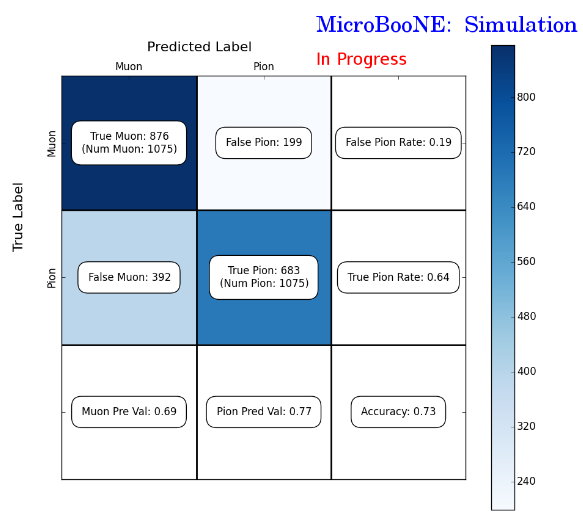
\includegraphics[width=\textwidth,height=3in]{figs/confusion1_train.png}
	\caption{Confusion Matrix showing Accuracy of CNN1075 using training MC data}
	\end{subfigure}
	\quad
	\begin{subfigure}[b]{.6\textwidth}
	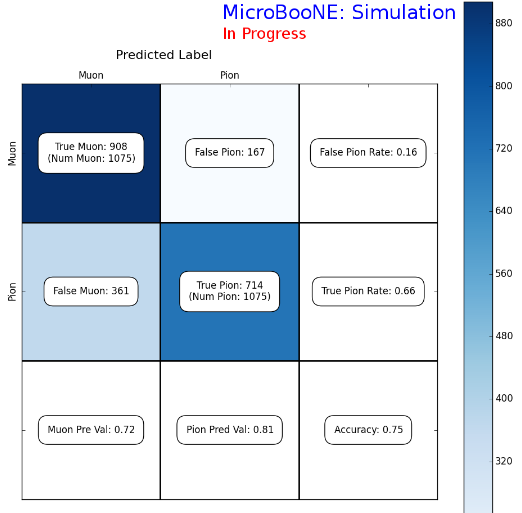
\includegraphics[width=\textwidth,height=3in]{figs/confusion1_test.png}
	\caption{Confusion Matrix showing Accuracy of CNN1075 using testing MC data}
	\end{subfigure}
	\quad
\caption{Description of confusion matrix variables: False pion rate = $false \pi/ total \pi$ True pion rate = $true \pi/total \pi$ Accuracy = $(true \pi rate + true \mu rate)/2$ Pion prediction value = $true \pi/(true \pi + false \pi)$ Muon prediction value = $true \mu/(true \mu + false \mu)$}
\label{fig:confusion1075}
\end{figure}

The confusion matrices shown in figure \ref{fig:confusion1075} show the accuracy for both the training and testing datasets. The fact that these two have similar accuracies is important because if the training dataset had a much higher accuracy, that indicates an over-training of the training sample which means the neural network didn't learn features to separate muons from pions, it just memorized what was in the training dataset. Also note that the neural network does a better job of identifying muons than pions. This can be attributed to the more complex event scenes pions tend to leave in the detector due to pion interacting more in LAr than muons do. The CNN may do better at identifying pions with a larger training sample.

\subsection{Training CNN10000}
The hyperparameters used for CNN10000 are shown below. The batch size for the training and testing as well as the test{\_}iter were chosen to encompass the whole training/testing image set when doing accuracy/loss calculations. To do this, multiplying the test{\_}iter by the test batch size gives you the amount of images used when calculating accuracy/loss curves. 

\begin{multicols}{3}
\begin{itemize}
 \item \textit{train{\_}batch{\_}size: 100}
 \item \textit{test{\_}batch{\_}size: 100}
 \item \textit{test{\_}iter: 100}
 \item \textit{test{\_}interval: 100}
 \item \textit{base{\_}lr: 0.001}
 \item \textit{lr{\_}policy: "step"}
 \item \textit{gamma: 0.1}
 \item \textit{stepsize: 1000}
 \item \textit{display: 100}
 \item \textit{max{\_}iter: 10000}
 \item \textit{momentum: 0.99}
 \item \textit{weight{\_}decay: 0.0005}
 \item \textit{snapshot: 100}
\end{itemize}
\end{multicols}

\begin{figure}[htp!]
\centering
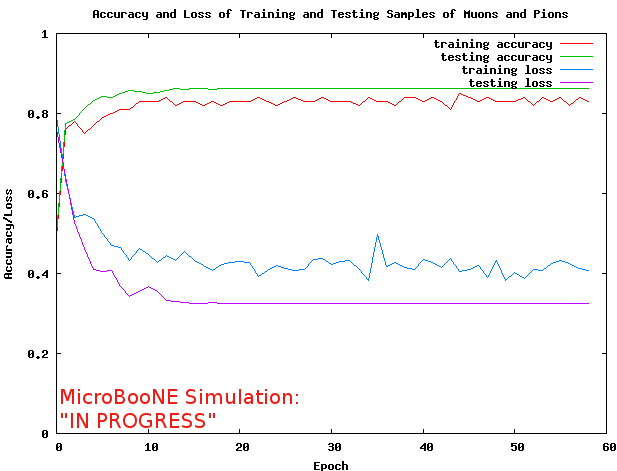
\includegraphics[width=\textwidth]{figs/acc_loss_10000_062117.png}
\caption{Accuracy vs. Loss of AlexNet 2-output $\mu/\pi$ sample consisting of 10,000 images each.} 
\label{fig:loss_accuracy}
\end{figure}

The same architecture that was used to train CNN1075 was employed on CNN10000, AlexNet. Caffe \cite{caffe} was the software package used for both CNNs. The differences include batch size and test{\_}iter and momentum to account for the larger dataset. Figure \ref{fig:loss_accuracy} shows the loss and accuracy of CNN10000. There is around a 10\% increase in accuracy from CNN1075 to CNN10000, 85\%, and around a 20\% decrease in loss, 36\%.

\begin{figure}[htp!]
\centering
	\begin{subfigure}[b]{.7\textwidth}
	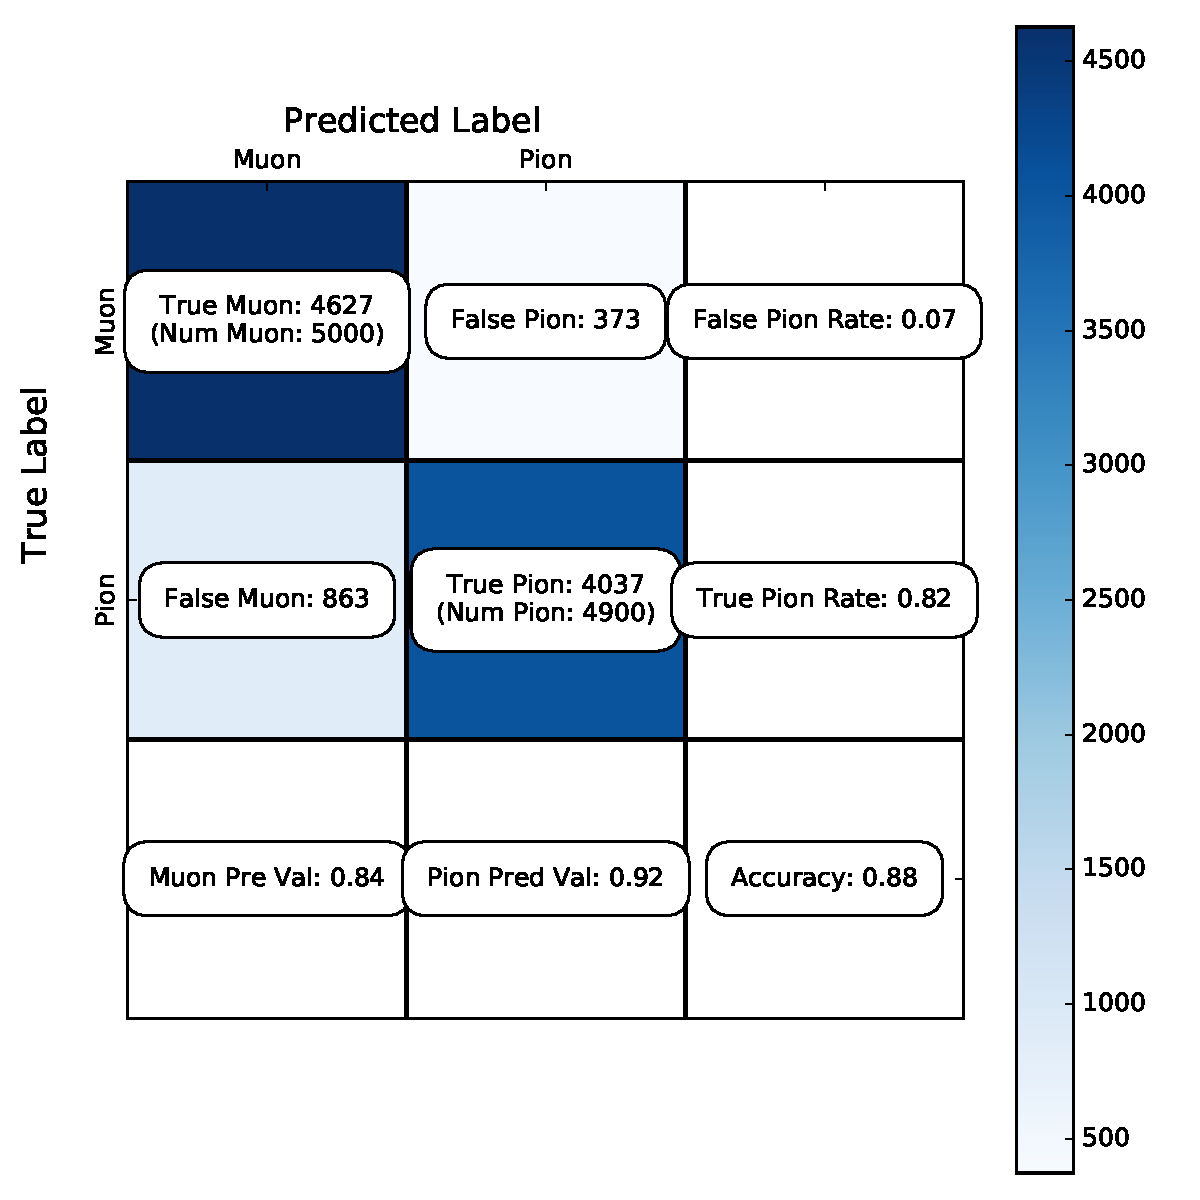
\includegraphics[width=\textwidth,height=3.5in]{figs/train_confusion.pdf}
	\caption{Confusion Matrix showing Accuracy of CNN10000 using training MC data}
	\label{fig:confusion}
	\end{subfigure}
	\quad
	\begin{subfigure}[b]{.7\textwidth}
	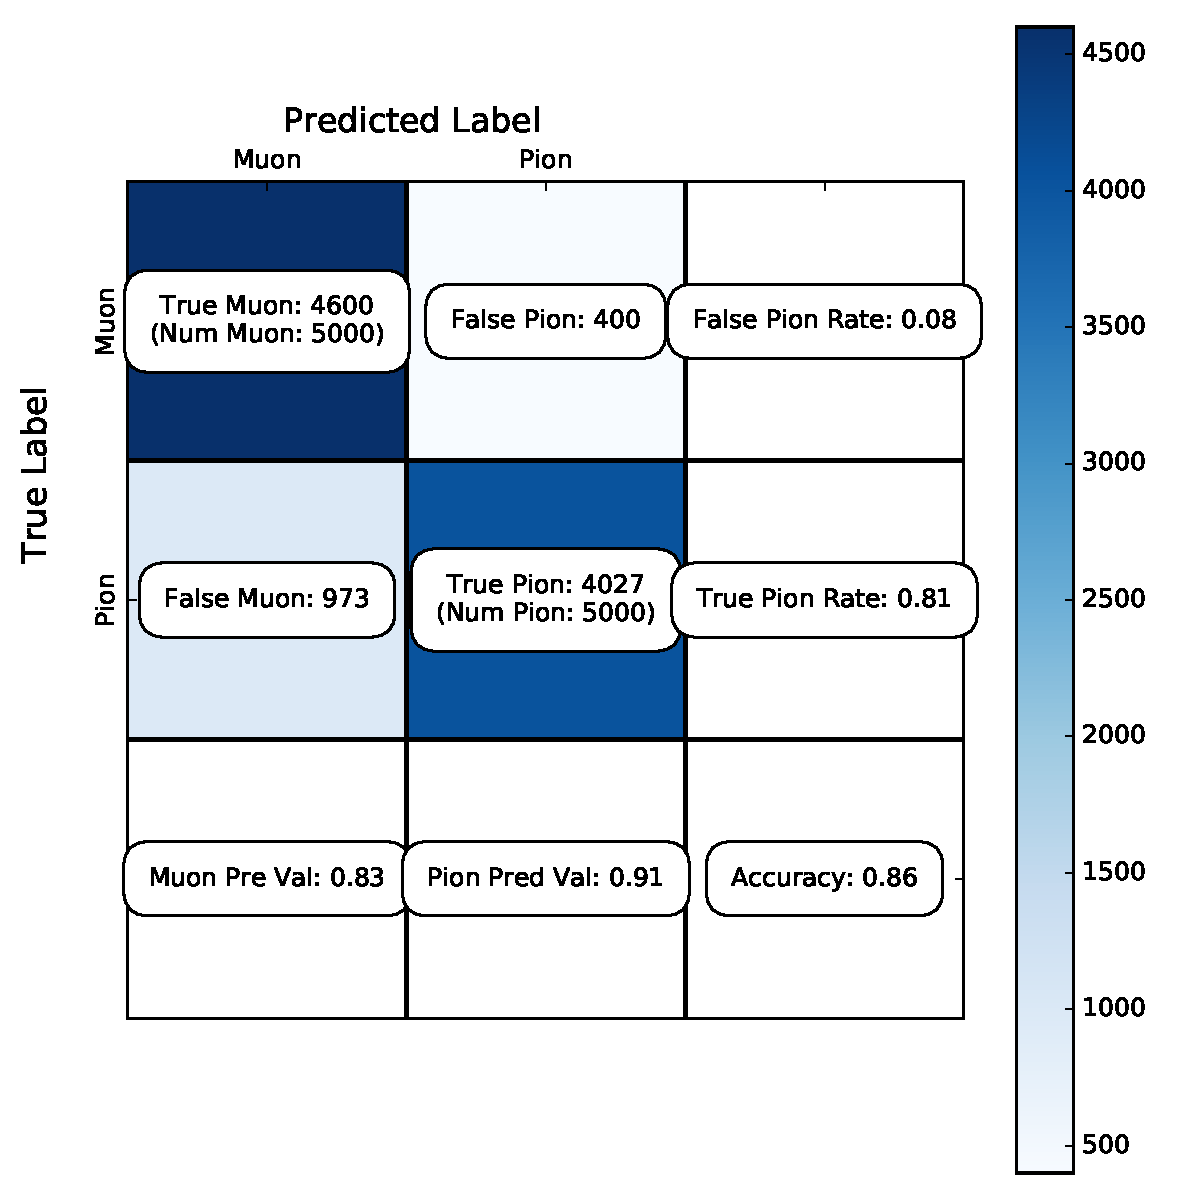
\includegraphics[width=\textwidth,height=3.5in]{figs/val_confusion.pdf}
	\caption{Confusion Matrix showing Accuracy of CNN10000 using testing MC data}
	\label{fig:confusion_test}
	\end{subfigure}
	\quad
\caption{Description of confusion matrix variables: False pion rate = $false \pi/ total \pi$; True pion rate = $true \pi/total \pi$; Accuracy = $(true \pi rate + true \mu rate)/2$; Pion prediction value = $true \pi/(true \pi + false \pi)$; Muon prediction value = $true \mu/(true \mu + false \mu)$}
\label{fig:CNN_train}
\end{figure}
\begin{figure}[htp!]
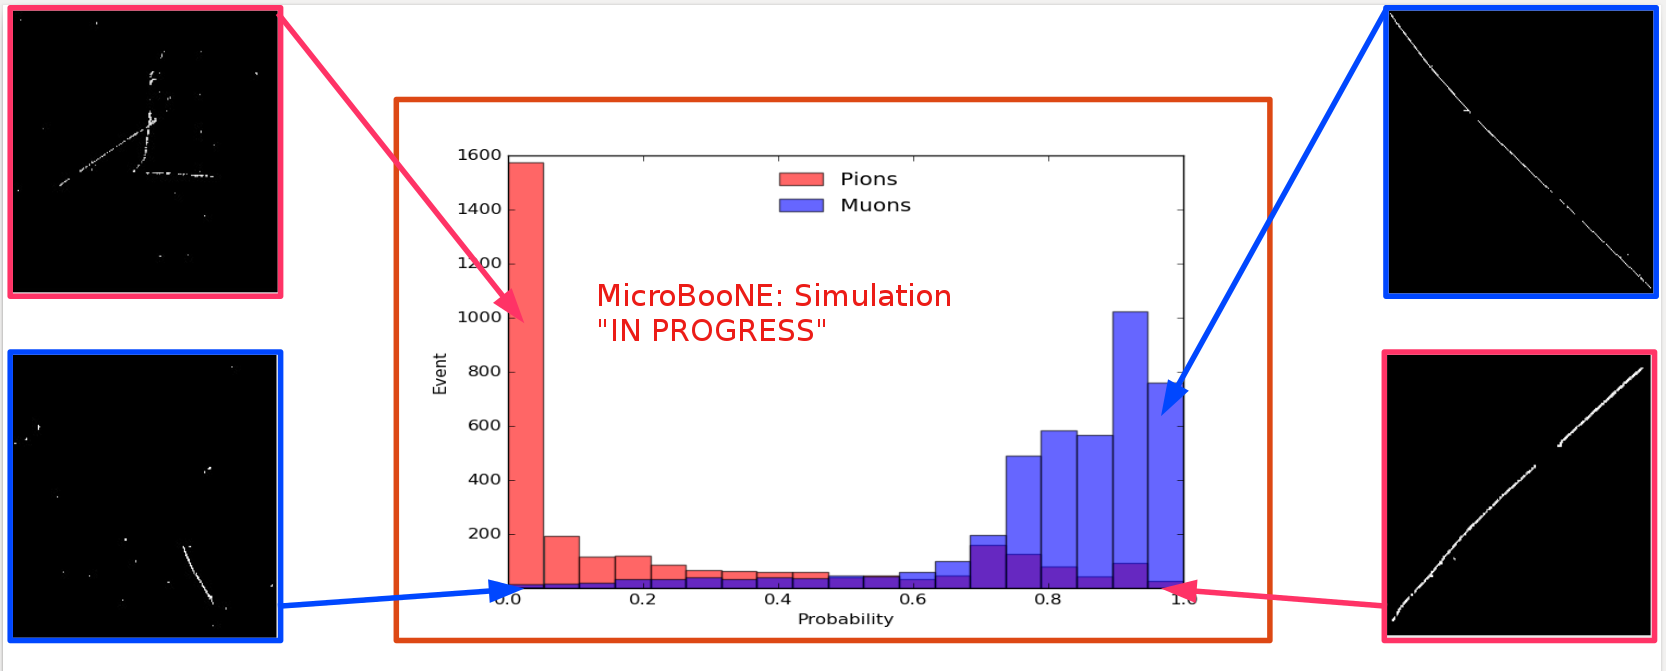
\includegraphics[width=\textwidth]{figs/mitch_hw.png}
\caption{Probability plot of muons and pions from testing set. Images surrounding histogram are a random event from lowest bin and highest bin for each particle.}
\label{fig:prob_plot}
\end{figure}

Figure \ref{fig:CNN_train} show a breakdown of $\mu/\pi$ separation for CNN10000. It also shows the network is not being over-trained due to the Accuracy of both the training and testing datasets being within .01\% of each-other. Figure \ref{fig:prob_plot} shows how well the neural network is doing at $\mu/\pi$ separation with respect to muon probability. The red bins corresponds to true pions and the blue bins correspond to true muons. There is still pion contamination in the high muon probability bins but by choosing a muon probability of $\geq 80\%$ we can reduce this. The CNNs increase in total accuracy can be attributed to an increase in accurately classifying pions as pions as seen in both the confusion matrix in figure \ref{fig:CNN_train} and the large number of events in the zero bin of the muon probability plot seen in figure \ref{fig:prob_plot} that corresponds to high probability pions.   



\subsection{Training CNN100000}
CNN100000 used the GoogleNet architecture rather than the AlexNet architecture used in the two previous trained CNNs. This is the first time the neural network was trained on a larger particle class, $\mu/\pi/p/\gamma/e$, and on higher resolution images. This CNN also employed GPUs during the training process. The hyperparameters are shown below:

\begin{multicols}{3}
\begin{itemize}
 \item \textit{train{\_}batch{\_}size: 18}
 \item \textit{test{\_}batch{\_}size: 2}
 \item \textit{test{\_}iter: 2000}
 \item \textit{test{\_}interval: 2000}
 \item \textit{base{\_}lr: 0.001}
 \item \textit{lr{\_}policy: "step"}
 \item \textit{gamma: 0.96}
 \item \textit{stepsize: 10000}
 \item \textit{average{\_}loss: 40}
 \item \textit{display: 40}
 \item \textit{max{\_}iter: 10000}
 \item \textit{momentum: 0.99}
 \item \textit{weight{\_}decay: 0.0002}
 \item \textit{snapshot: 50000}
\end{itemize}
\end{multicols}


\begin{figure}[htp!]
\centering
\includegraphics[width=.8\textwidth]{../images/GPU_9010split_hires_iterations_alldata_allparticle.png}
\caption{Training and testing accuracy of CNN trained on 100,000 images of \mu/\pi/p/\gamma/e with 20,000 images of each particle. Each image was a size of 576x576 and the images per particle were split 90\% use for training and 10\% used for testing the network}
\label{fig:gpuacc}
\end{figure}

\begin{figure}[htp!]
\centering
\includegraphics[width=.8\textwidth]{../images/GPU_9010split_hires_iterations_alldata_allparticle_loss.png}
\caption{Training and testing loss of CNN trained on 100,000 images of \mu/\pi/p/\gamma/e}
\label{fig:gpuloss}
\end{figure}
The accuracy and loss for CNN100000 are shown in figures \ref{fig:gpuacc} and \ref{fig:gpuloss}. The jumps shown in both figures are when the training was stopped to fine-tune the weight decay and the learning rate. The accuracy leveled off at \sim 80\% and the loss was at \sim 0.48. 



\begin{figure}[htp!]
\centering
\includegraphics[width=\textwidth]{../images/confusion_allparticle_v3.pdf}
\caption{Confusion Matrix of all five particles }
\label{fig:confusion100000}
\end{figure}
Figure \ref{fig:confusion100000} shows the confusion matrix of CNN100000. The proton identification of the neural network is at 85\% and the highest out of all five particles. One thing to note is clear separation between particles that leave track like objects in the MicroBooNE detector, $\mu/\pi/p$, versus particles that leave shower like objects in MicroBooNE, $e/\gamma$. 



\begin{figure}[htp!]
\centering
\includegraphics[width=.8\textwidth]{../csv_output/true_labels_1102.png}
\caption{t-SNE of CNN}
\label{fig:tsne}
\end{figure}
Another visualization of how the neural network is learning is shown in \ref{fig:tsne}.  t-SNEs \cite{tsne} is a technique used for dimensionality reduction developed for use in visualizing high-dimensional datasets. Each datapoint is given a location in a two or three-dimensional map by using stochastic neighbor embedding to convert high-dimensional euclidean distances between datapoints into conditional probabilities that represent the similarities between these datapoints. For datapoints close together on the map, their conditional probabilities are high, for datapoints with a wide separation between them, their conditional probabilities are very small. Figure \ref{fig:tsne} is a t-SNE of the final training iteration of a subset of the training sample used in CNN100000. You can see a clear separation between track like objects and shower like objects. You can also see that electrons and gammas are not as separated as muons, pions, and protons. For the purpose of this thesis, this isn't an issue but later iterations of training could include more images for the gamma and electron classes to help the CNN further separate these classes.


\begin{figure}
\centering
	\begin{subfigure}[b]{.475\textwidth}
		\centering
		\includegraphics[width=\textwidth]{../csv_output/muon_prob.png}
		\caption{Muon Prob}
		\label{fig:muonprob}
	\end{subfigure}
	\begin{subfigure}[b]{.475\textwidth}
		\centering
		\includegraphics[width=\textwidth]{../csv_output/pi_prob.png}
		\caption{Pion Prob}
		\label{fig:piprob}
	\end{subfigure}
	\begin{subfigure}[b]{.475\textwidth}
		\centering
		\includegraphics[width=\textwidth]{../csv_output/pi_prob.png}
		\caption{Proton Prob}
	\label{fig:piprob}
	\end{subfigure}
	\begin{subfigure}[b]{.475\textwidth}
		\centering
		\includegraphics[width=\textwidth]{../csv_output/eminus_prob.png}
		\caption{Electron Prob}
		\label{fig:eminusprob}
	\end{subfigure}
	\begin{subfigure}[b]{.475\textwidth}
		\centering
		\includegraphics[width=\textwidth]{../csv_output/gamma_prob.png}
		\caption{Gamma Prob}
		\label{fig:gammaprob}
	\end{subfigure}
\caption{Probabilities of different particle classes as well as their contamination from other classes}
\label{fig:particleprob}
\end{figure}
Figure \ref{fig:particleprob} shows the probability of each particle class and the highest probability misidentification for each class. For muons, the largest misidentification is from protons. For pions, both protons and muons get misidentified as pions at around the same probability. Similar behavior is also seen for proton identification. Electrons and gammas are misidentified as each-other with similar probabilities.  



\begin{figure}[htp]
\centering
\includegraphics[width=.8\linewidth=]{../csv_output/prob_allparticle_normalized.pdf}
\caption{Muon probability of true muons (blue) versus pions (red), protons (cyan), gammas (green) and electrons (magenta).}
\label{fig:prob}
\end{figure}
To see what type of background contamination one would be dealing with when doing muon identification, muon probabilities for each particle class was plotted against the probability of true muons to see how well muon signal vs other particle background separation can be done with CNN100000. Figure \ref{fig:prob} is showing the true muon probability for true muons, versus the rest of the particle classes. This plot describes which muon probability value should be chosen for the least amount of other particle contamination. For electrons and gammas, a muon probability of \sim 75\% would eliminate $e/\gamma$ contamination. For pions and protons, there is contamination at all values of muon probability, but the contamination is drastically reduced at a muon probability $\geq 75\%$.
 
One of the main concerns with training a neural network was that the features the network would learn to separate muons from pions would be track range, which is what was used to begin with in selection I. To make sure that wasn't the case, the next thing that was looked at was the muon probability versus track range and momentum of the track. Figures \ref{fig:mupi_kinematics} through \ref{fig:mug_kinematics} show the muon probability in blue for all plots against all other particles. A zoomed in version of track range for all particles was also plotted to make sure there is separation between the particles at low track range. The $\mu/\pi$ separation in track range and momentum is less than for $p/e/\gamma$ but that was to be expected. Although the separation isn't as good as the other particles, there still is separation at low momentum and low track range which cannot be done by using a track range cut like selection I does.  
\begin{figure}[htp]
\centering
	\begin{subfigure}[t]{.475\textwidth}
		\centering
		\includegraphics[width=\textwidth]{../csv_output/mu_pi_acc_tracklength_all.pdf}
		\caption{Track range versus muon probability for true muons (blue) and true pions (red).}
		\label{fig:mupi_tracklength}
	\end{subfigure}
	\begin{subfigure}[t]{.475\textwidth}
		\centering
		\includegraphics[width=\textwidth]{../csv_output/mu_pi_acc_tracklength_75.pdf}
		\caption{Track range $\leq 75$ cm versus muon probability for true muons (blue) and true pions (red).}
		\label{fig:mupi_tracklength75}
	\end{subfigure}
	\begin{subfigure}[t]{.475\textwidth}
		\centering
		\includegraphics[width=\textwidth]{../csv_output/mu_pi_acc_momentum.pdf}
		\caption{Momentum versus muon probability for true muons (blue) and true pions (red).}
		\label{fig:mupi_momentum}
	\end{subfigure}
\caption{Kinematic distributions versus muon probability for true muons and true pions.}
\label{fig:mupi_kinematics}
\end{figure}

\begin{figure}[htp]
\centering
	\begin{subfigure}[b]{.475\textwidth}
		\centering
		\includegraphics[width=\textwidth]{../csv_output/mu_p_acc_tracklength_all.pdf}
		\caption{Track range versus muon probability for true muons (blue) and true protons (cyan).}
		\label{fig:mup_tracklength}
	\end{subfigure}
	\begin{subfigure}[b]{.475\textwidth}
		\centering
		\includegraphics[width=\textwidth]{../csv_output/mu_p_acc_tracklength_75.pdf}
		\caption{Track range $\leq 75$ cm versus muon probability for true muons (blue) and true protons (cyan).}
		\label{fig:mup_tracklength75}
	\end{subfigure}
	\begin{subfigure}[b]{.475\textwidth}
		\centering
		\includegraphics[width=\textwidth]{../csv_output/mu_p_acc_momentum.pdf}
		\caption{Momentum versus muon probability for true muons (blue) and true protons (cyan).}
		\label{fig:mup_momentum}
	\end{subfigure}
\caption{Kinematic distributions versus muon probability for true muons and true protons.}
\label{fig:mup_kinematics}
\end{figure}

\begin{figure}[htp]
\centering
	\begin{subfigure}[b]{.475\textwidth}
		\centering
		\includegraphics[width=\textwidth]{../csv_output/mu_e_acc_tracklength_all.pdf}
		\caption{Track range versus muon probability for true muons (blue) and true electrons (magenta).}
		\label{fig:mup_tracklength}
	\end{subfigure}
	\begin{subfigure}[b]{.475\textwidth}
		\centering
		\includegraphics[width=\textwidth]{../csv_output/mu_e_acc_tracklength_75.pdf}
		\caption{Track range $\leq 75$ cm versus muon probability for true muons (blue) and true electrons (magenta).}
		\label{fig:mup_tracklength75}
	\end{subfigure}
	\begin{subfigure}[b]{.475\textwidth}
		\centering
		\includegraphics[width=\textwidth]{../csv_output/mu_e_acc_momentum.pdf}
		\caption{Momentum versus muon probability for true muons (blue) and true electrons (magenta).}
		\label{fig:mup_momentum}
	\end{subfigure}
\caption{Kinematic distributions versus muon probability for true muons and true electrons.}
\label{fig:mue_kinematics}
\end{figure}

\begin{figure}[htp]
\centering
	\begin{subfigure}[b]{.475\textwidth}
		\centering
		\includegraphics[width=\textwidth]{../csv_output/mu_g_acc_tracklength_all.pdf}
		\caption{Track range versus muon probability for true muons (blue) and true gammas (green).}
		\label{fig:mup_tracklength}
	\end{subfigure}
	\begin{subfigure}[b]{.475\textwidth}
		\centering
		\includegraphics[width=\textwidth]{../csv_output/mu_g_acc_tracklength_75.pdf}
		\caption{Track range $\leq 75$ cm versus muon probability for true muons (blue) and true gammas (green).}
		\label{fig:mup_tracklength75}
	\end{subfigure}
	\begin{subfigure}[b]{.475\textwidth}
		\centering
		\includegraphics[width=\textwidth]{../csv_output/mu_g_acc_momentum.pdf}
		\caption{Momentum versus muon probability for true muons (blue) and true gammas (green).}
		\label{fig:mup_momentum}
	\end{subfigure}
\caption{Kinematic distributions versus muon probability for true muons and true gammas.}
\label{fig:mug_kinematics}
\end{figure}


